% !TeX spellcheck = ru_RU-Russian

\documentclass{beamer}
\mode<presentation>
\usetheme{Ilmenau}

\setbeameroption{show notes on second screen}

\author{Василий Генералов \\ VSGeneralov@sberbank.ru}
\title{Machine Learning 101}

\usepackage[utf8]{inputenc}
\usepackage[T1,T2A]{fontenc}
\usepackage{hyperref}
\hypersetup{colorlinks=true,pageanchor=true}
\usepackage{tikz}
\usetikzlibrary{fit}
\usepackage{pgfplots}
\pgfplotsset{compat=newest}
\usepackage{amsmath}

%%% dude wtf
\usepackage{fancyvrb}
\makeatletter
\def\KV@FV@lastline@default{%
  \let\FancyVerbStopNum\m@ne
\let\FancyVerbStopString\relax}
\fvset{lastline}
\makeatother
\usepackage{minted}
%%%

\def \MinSize {22}
\def \TikzScale {0.7}

\DeclareMathOperator*{\argmin}{argmin}
\newcommand{\mtx}[1]{\boldsymbol{#1}}
\newcommand{\Loss}{\mathcal{L}}

\tikzstyle{neuron}=[
  draw=black,
  circle,
  minimum size=\MinSize
]

\begin{document}

\begin{frame}
  \maketitle
\end{frame}

\begin{frame}
  \tableofcontents
\end{frame}

\section{Модель нейрона}

\begin{frame}{\secname : \subsecname}
  \framesubtitle{Сумматор}

  \note{Поговорим про <<нейро>> в нейросетях. Из слова понятно, что
    это сети нейронов. А что такое нейрон?~--- из них состоит наш с
    вами мозг, такие нейроны назовем биологическими.
    Биологический нейрон реагирует на спайки~--- импульсы,
    приходящие на аксоны. Нейросети же содержат модели нейронов,  но
    импульсное поведение сложно моделировать.
    Самой удобной моделью оказался линейный сумматор. Слева на слайде
    можно видеть выражение, описывающее модель, а справа~--- ее
    графическую интерпретацию.    Множество $w_i$
  принято называть весами нейрона, а свободный член $b$~--- смещением.}

  \begin{columns}

    \begin{column}{0.5\textwidth}
      $$ y = \sum_{i}^{} w_i \cdot x_i + b $$
    \end{column}

    \begin{column}{0.5\textwidth}
      \begin{center}
        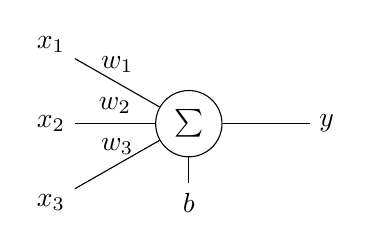
\begin{tikzpicture}
          \def \x {3}
          \def \y {0}
          \def \xOff {1.75}
          \def \yOff {1}

          \node[neuron] (n1) at (\x, \y) {$\sum$};

          % ins
          \node (x1) at (\x - \xOff, \y + \yOff) {$x_1$};
          \node (x2) at (\x - \xOff, \y) {$x_2$};
          \node (x3) at (\x - \xOff, \y - \yOff) {$x_3$};
          \node (b1) at (\x, \y - \yOff) {$b$};

          % out
          \node (y1) at (\x + \xOff, \y) {$y$};

          % connect ins
          \foreach \i in {1,...,3}{
            \draw (x\i) -- (n1) node[midway,above] {$w_\i$};
          }
          \draw (b1) -- (n1);

          % connect out
          \draw (n1) -- (y1);
        \end{tikzpicture}
      \end{center}
    \end{column}

  \end{columns}
\end{frame}

\section{Линейный слой}

\begin{frame}{\secname : \subsecname}
  \framesubtitle{Полносвязный слой, fully connected, linear}

  \note{Если объединить два слоя нейронов и соединить каждый выход с
    каждым входом, то получится линейный слой, также называемый
    полносвязным. Количество нейронов в первом слое принято называть
    шириной входа, а во втором~--- шириной выхода. Функцию линейного
    слоя можно описать произведением матрицы весов на вектор входных
    параметров. На этом слайде снова математическое описание модели
    слева и графический аналог справа. Вспомним выражение для линейной
    функции $a \cdot x + b$. Оно очень похоже на описание линейного
  слоя. Попробуем воспроизвести поведение функции через слой.}

  \begin{columns}

    \begin{column}{0.5\textwidth}
      $$
      y = x \cdot \mtx{A}^T + \mtx{b}
      $$
      где $\mtx{A}[O \times I]$~--- матрица обучаемых весов,
      $\mtx{b}[O]$~--- вектор обучаемых смещений,
      подробнее в
      \href{https://docs.pytorch.org/docs/stable/generated/torch.nn.Linear.html}{документации}

    \end{column}

    \begin{column}{0.5\textwidth}
      \begin{center}
        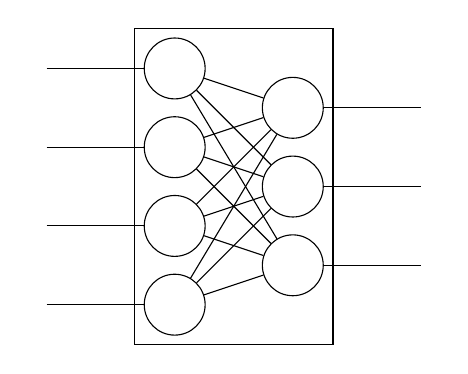
\begin{tikzpicture}
          \def \InSize {3}
          \def \OutSize {2}

          \def \OffX {1.75}

          \def \InX {0}
          \def \InY {-3}
          \def \OffInY {1}

          \def \OutX {1.5}
          \def \OutY {-2.5}
          \def \OffOutY {1}

          \foreach \i in {0,...,\InSize}{
            \def \y {\InY + \i * \OffInY}
            \node[neuron] (n\i) at (\InX, \y) {};
            \node (x\i) at (\InX - \OffX, \y) {};
            \draw (x\i) -- (n\i);
          }

          \foreach \i in {0,...,\OutSize}{
            \def \y {\OutY + \i * \OffOutY}
            \node[neuron] (m\i) at (\OutX, \y) {};
            \node (z\i) at (\OutX + \OffX, \y) {};
            \draw (z\i) -- (m\i);
          }

          \foreach \i in {0,...,\InSize}{
            \foreach \j in {0,...,\OutSize}{
              \draw (n\i) -- (m\j);
            }
          }

          \node[draw, fit=(n0) (n\InSize) (m0) (m\OutSize)] {};
        \end{tikzpicture}
      \end{center}
    \end{column}

  \end{columns}
\end{frame}

\begin{frame}[fragile]{\secname : \subsecname}
  \framesubtitle{Описание модели}

  \note{Выразим нашу идею с помощью PyTorch. Очевидно, что
    использование фреймворка прячет от пользователя львиную долю кода.
    Но даже с учетом этого, простейшая модель занимает 3 строчки~---
  конструктор и метод прямого прохода.}

  \inputminted[firstline=19,lastline=25]{python}{linear_regression_1/linear_regression_1.py}
\end{frame}

\begin{frame}{\secname : \subsecname}
  \framesubtitle{Регрессия линейной функции}

  \note{Слева синим изображены исходная функция и легкий шум,
    наложенный на ее значения. Красная линия~--- восстановленная
    моделью зависимость. Как видно, в области значений, которые
    <<видела>> модель, алгоритм неплохо приблизил функцию. График
    справа показывает ошибку модели по мере работы алгоритма. В
    машинном обучении <<эпохой>> принято называть одну итерацию цикла
  <<оценка-ошибка-коррекция>>.}

  \begin{columns}

    \begin{column}{0.5\textwidth}
      \begin{tikzpicture}[scale=\TikzScale]
        \begin{axis}[title=Результат регрессии,xlabel=$x$,ylabel=$y$,legend
          entries={Исходная функция,Исходная функция + шум,Предсказание модели}]
          \addplot[blue] table[x=X,y=Y,col sep=comma]
          {linear_regression_1/output.csv};
          \addplot[blue,only marks,mark size=1] table[x=X,y=Ynoise,col
          sep=comma] {linear_regression_1/output.csv};
          \addplot[red] table[x=X,y=Ypred,col sep=comma]
          {linear_regression_1/output.csv};
        \end{axis}
      \end{tikzpicture}
    \end{column}

    \begin{column}{0.5\textwidth}
      \begin{tikzpicture}[scale=\TikzScale]
        \begin{axis}[title=Потери,xlabel=Эпоха,ylabel=MSE,legend
          entries={Валидация,Обучение}]
          \addplot[blue] table[col sep=comma]
          {linear_regression_1/test_loss.csv};
          \addplot[red] table[col sep=comma]
          {linear_regression_1/train_loss.csv};
        \end{axis}
      \end{tikzpicture}
    \end{column}

  \end{columns}
\end{frame}

\begin{frame}{\secname : \subsecname}
  \framesubtitle{Регрессия произвольной функции}

  \note{Имея на руках способ выучить закономерности из данных,
    появляется желание исследовать что-то более сложное. Для примера
    возьмем синус и как в прошлый раз добавим шум. На правом графике
    видно, как ошибка не может стабилизироваться, да и предсказание
    модели напоминает синус очень слабо. Эта картина не изменится ни от
    большего количества слоев, ни от дополнительных параметров, ни от
    новых данных. Действительно, линейная модель может выучить только
  линейный закон. Так что же делать с нелинейными данными?}

  \begin{columns}
    \begin{column}{0.5\textwidth}
      \begin{tikzpicture}[scale=\TikzScale]
        \begin{axis}[title=Результат регрессии,xlabel={$x$,
            $^{\circ}$},ylabel=$y$,legend
          entries={Исходная функция,Исходная функция + шум,Предсказание модели}]
          \addplot[blue] table[x=X,y=Y,col sep=comma]
          {linear_regression_2/output.csv};
          \addplot[blue,only marks,mark size=1] table[x=X,y=Ynoise,col
          sep=comma] {linear_regression_2/output.csv};
          \addplot[red] table[x=X,y=Ypred,col sep=comma]
          {linear_regression_2/output.csv};
        \end{axis}
      \end{tikzpicture}
    \end{column}

    \begin{column}{0.5\textwidth}
      \begin{tikzpicture}[scale=\TikzScale]
        \begin{axis}[title=Потери,xlabel=Эпоха,ylabel=MSE,ymode=log,legend
          entries={Валидация,Обучение}]
          \addplot[blue] table[col sep=comma]
          {linear_regression_2/test_loss.csv};
          \addplot[red] table[col sep=comma]
          {linear_regression_2/train_loss.csv};
        \end{axis}
      \end{tikzpicture}
    \end{column}
  \end{columns}
\end{frame}

\section{Нелинейность}

\begin{frame}{\secname : \subsecname}
  \framesubtitle{Активация}

  \note{Ответ прост~--- нелинейность привносит активация. Для начала
    положим, что существует функция $g$, принимающая результат работы
    нейрона. Как обычно, слева и справа математическое и графическое
    представление. В некоторых источниках сочетание нейрон/линейный слой +
  активация называют <<перцептрон>>.}

  \begin{columns}

    \begin{column}{0.5\textwidth}
      $$
      y = g\left(\sum_{i}^{} w_i \cdot x_i + b\right)
      $$
      где $g(x)$~--- функция активации (Sigmoid, ReLU, $\tanh$, и т.д.)

    \end{column}

    \begin{column}{0.5\textwidth}
      \begin{center}
        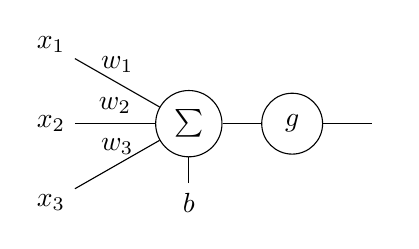
\begin{tikzpicture}
          \def \x {3}
          \def \y {0}
          \def \xOff {1.75}
          \def \yOff {1}

          \node[neuron] (n1) at (\x, \y) {$\sum$};

          \node (x1) at (\x - \xOff, \y + \yOff) {$x_1$};
          \node (x2) at (\x - \xOff, \y) {$x_2$};
          \node (x3) at (\x - \xOff, \y - \yOff) {$x_3$};
          \node (b1) at (\x, \y - \yOff) {$b$};

          \node[neuron] (y1) at (\x + 0.75 * \xOff, \y) {$g$};
          \node (y2) at (\x + 1.4 * \xOff, \y) {};

          \foreach \i in {1,...,3}{
            \draw (x\i) -- (n1) node[midway,above] {$w_\i$};
          }
          \draw (b1) -- (n1);

          \draw (n1) -- (y1);
          \draw (y1) -- (y2);
        \end{tikzpicture}
      \end{center}
    \end{column}

  \end{columns}
\end{frame}

\begin{frame}{\secname : \subsecname}
  \framesubtitle{Описание модели}

  \note{Не будем откладывать и добавим функцию активации~---
    сигмоиду~--- между линейными слоями. В коде снова требуется всего пара
  новых строчек.}

  \inputminted[firstline=19,lastline=30]{python}{linear_regression_3/linear_regression_3.py}
\end{frame}

\begin{frame}{\secname : \subsecname}
  \framesubtitle{Регрессия произвольной функции}

  \note{Вернемся к регрессии синуса. Картина слева далека от идеала,
    и модель можно обучать дальше, но
    результат уже принципиально лучше простой линии, что видно по выходящим
  на плато графикам потерь справа.}

  \begin{columns}
    \begin{column}{0.5\textwidth}
      \begin{tikzpicture}[scale=\TikzScale]
        \begin{axis}[title=Результат регрессии,xlabel={$x$,
            $^{\circ}$},ylabel=$y$,legend pos=north west,legend
            entries={\tiny{Исходная функция},\tiny{Исходная функция +
          шум},\tiny{Предсказание модели}}]
          \addplot[blue] table[x=X,y=Y,col sep=comma]
          {linear_regression_3/output.csv};
          \addplot[blue,only marks,mark size=1] table[x=X,y=Ynoise,col
          sep=comma] {linear_regression_3/output.csv};
          \addplot[red] table[x=X,y=Ypred,col sep=comma]
          {linear_regression_3/output.csv};
        \end{axis}
      \end{tikzpicture}
    \end{column}

    \begin{column}{0.5\textwidth}
      \begin{tikzpicture}[scale=\TikzScale]
        \begin{axis}[title=Потери,xlabel=Эпоха,ylabel=MSE,legend
          entries={Валидация,Обучение}]
          \addplot[blue] table[col sep=comma]
          {linear_regression_3/test_loss.csv};
          \addplot[red] table[col sep=comma]
          {linear_regression_3/train_loss.csv};
        \end{axis}
      \end{tikzpicture}
    \end{column}
  \end{columns}
\end{frame}

\begin{frame}{\secname : \subsecname}
  \framesubtitle{Sigmoid, ReLU}

  \note{Рассмотрим активации ближе. На слайде показаны две самые
    популярные из них~--- сигмоида и rectified linear unit. Первую
    применяют для предсказания вероятности одного из двух исходов,
    потому что ее значение лежит в пределах
    от 0 до 1. ReLU же можно часто встретить в
  сверточных сетях.}

  \begin{columns}

    \begin{column}{0.5\textwidth}
      \begin{tikzpicture}[scale=\TikzScale]
        \begin{axis}[title=Sigmoid,xlabel=$x$,ylabel=$g$,legend
          entries={$\frac{1}{1+ e^{-x}}$},legend pos=north west]
          \addplot[blue] table[x=X,y=Sigmoid,col sep=comma]
          {activation/output.csv};
        \end{axis}
      \end{tikzpicture}
    \end{column}

    \begin{column}{0.5\textwidth}
      \def \ReLU {$\max(0,x)$}
      \begin{tikzpicture}[scale=\TikzScale]
        \begin{axis}[title=ReLU,xlabel=$x$,ylabel=$g$,legend
          entries={\ReLU},legend pos=north west]
          \addplot[blue] table[x=X,y=ReLU,col sep=comma]
          {activation/output.csv};
        \end{axis}
      \end{tikzpicture}
    \end{column}

  \end{columns}
\end{frame}

\begin{frame}{\secname : \subsecname}
  \framesubtitle{$\tanh$, GELU}

  \note{Еще один вариант~--- гиперболический тангенс, его применяли
    в первых сверточных сетях. Последняя функция~--- GELU,
    она учитывает не
    только значения входа, но и статистику через $\Phi(x)$~---
    функцию распределения. Значение $\Phi(x)$ равняется
    вероятности, с которой случайная величина из нормального
  распределения меньше либо равна $x$.}

  \begin{columns}

    \begin{column}{0.5\textwidth}
      \begin{tikzpicture}[scale=\TikzScale]
        \begin{axis}[title=$\tanh$,xlabel=$x$,ylabel=$g$,legend
          entries={$\tanh(x)$},legend pos=north west]
          \addplot[blue] table[x=X,y=tanh,col sep=comma]
          {activation/output.csv};
        \end{axis}
      \end{tikzpicture}
    \end{column}

    \begin{column}{0.5\textwidth}
      \begin{tikzpicture}[scale=\TikzScale]
        \begin{axis}[title=GELU,xlabel=$x$,ylabel=$g$,legend
          entries={$x \cdot \Phi(x)$},legend pos=north west]
          \addplot[blue] table[x=X,y=GELU,col sep=comma]
          {activation/output.csv};
        \end{axis}
      \end{tikzpicture}
    \end{column}

  \end{columns}
\end{frame}

\begin{frame}{\secname : \subsecname}
  \framesubtitle{Другие функции активации}

  \note{Мы рассмотрели сигмоиду, ReLU, гиперболический тангенс, GELU.
  Другие функции можно найти в документации фреймворка PyTorch.}

  \begin{itemize}
    \item \textbf{Sigmoid}
    \item \textbf{ReLU}
    \item $\boldsymbol{\tanh}$
    \item \textbf{GELU}
    \item LogSigmoid
    \item PReLU
    \item LeakyReLU
    \item больше в
      \href{https://docs.pytorch.org/docs/stable/nn.html\#non-linear-activations-weighted-sum-nonlinearity}{документации}
  \end{itemize}
\end{frame}

\section{Обучение}

\begin{frame}{\secname : \subsecname}
  \framesubtitle{Простейший цикл}

  \note{Цикл обучения уже был вскользь упомянут. Здесь мы выбираем
    функцию потерь и оптимизатор, речь о которых пойдет позже. В цикле
    мы делаем прямой проход модели, а затем оцениваем, насколько
    результаты далеки от правды. После чего на основе оценки обновляем
  обучаемые параметры.}

  \inputminted[firstline=42,lastline=50]{python}{linear_regression_1/linear_regression_1.py}
\end{frame}

\begin{frame}{\secname : \subsecname}
  \framesubtitle{Функция потерь}
  Критерий обученности модели~--- значение функции потерь $\Loss$.
  Задача обучающего цикла~--- минимизация ее значения:
  $$
  \argmin_{\mtx{W}}\Loss\left(\mtx{Y}^{\ell},\mtx{Y}\left(\mtx{X},\mtx{W}\right)\right)
  $$
  где $\mtx{Y}^{\ell}$~--- истинное значение из датасета,
  $\mtx{Y}$~--- предсказание модели, $\mtx{X}$, $\mtx{W}$~--- входные
  данные и обученные веса модели
\end{frame}

\begin{frame}{\secname : \subsecname}
  \framesubtitle{MSE, MAE}
  Для задач регрессии используются Mean Squared Error Loss:
  $$
  MSELoss = \frac{1}{n}\cdot\sum_{i}^{n}\left(y^{\ell}_i - y_i\right)
  $$
  и Mean Absolute Error Loss:
  $$
  L1Loss = \frac{1}{n} \cdot \sum_{i}^{n}\lvert y^{\ell}_i - y_i\rvert
  $$
\end{frame}

\begin{frame}{\secname : \subsecname}
  \framesubtitle{Cross Entropy, BCE}

  \note{Потери при классификации на несколько классов можно оценить с
    помощью cross entropy, дробь под логарифмом~--- вероятность от 0 до
    1, что данные относятся к $i$-му классу. Для бинарной классификации
  удобен частный случай~--- binary cross entropy.}

  В задачах классификации применяется Cross Entropy Loss:
  $$
  CrossEntropyLoss = -\sum_{i}^{c} y^{\ell}_i \cdot \log\frac{e^{y_{i}}}{
  \sum_{j}^{c} e^{y_{j}}}
  $$
  Частный случай~--- Binary Cross Entropy:
  $$
  BCELoss = -\left( y^{\ell}_i \cdot \log \left( y_i \right) + \left(
  1-y^{\ell}_i \right) \cdot \log \left(1 - y_i \right) \right)
  $$
\end{frame}

\begin{frame}{\secname : \subsecname}
  \framesubtitle{Другие функции потерь}

  \note{Функция потерь отражает обученность модели, желательно, чтобы
    она включала какую-то метрику реального применения модели, но это
  не всегда так. Больше по ссылке.}

  \begin{itemize}
    \item \textbf{MSELoss}
    \item \textbf{L1Loss}
    \item \textbf{CrossEntropyLoss}
    \item \textbf{BCELoss}
    \item CTCLoss
    \item NLLLoss
    \item PoissonNLLLoss
    \item больше в
      \href{https://docs.pytorch.org/docs/stable/nn.html\#loss-functions}{документации}
  \end{itemize}
\end{frame}

\begin{frame}{\secname : \subsecname}
  \framesubtitle{Минимизация значения функции}

  \note{Уже упомянуто, что цель обучения~--- минимизация функции
    потерь. Как это сделать? Если представить точку на параболе, то в
    крайнем случае можно подвинуть ее влево или вправо, оценить новое
    значение и выбрать, в каком направлении функция уменьшается. А
    куда двигать точку на рисунке справа? Направлений движения
  бесконечно много, и простого перебора недостаточно. Как же искать минимум?}

  \begin{columns}
    \begin{column}{0.5\textwidth}
      \begin{tikzpicture}[scale=\TikzScale]
        \begin{axis}[xlabel=$x$,ylabel=$y$]
          \addplot[blue] table[col sep=comma]
          {optimization_1/output2d.csv};
          \node[draw=red,circle,fill=red] at (-5, 25) {};
        \end{axis}
      \end{tikzpicture}
    \end{column}

    \begin{column}{0.5\textwidth}
      \begin{tikzpicture}[scale=\TikzScale]
        \begin{axis}[xlabel=$x$,ylabel=$y$,zlabel=$z$]
          \addplot3[surf,mesh/rows=50,shader=interp] table[col
          sep=comma] {optimization_1/output3d.csv};
          \node[circle,draw=red,fill=red] at (-5, -5, 50) {};
        \end{axis}
      \end{tikzpicture}
    \end{column}
  \end{columns}
\end{frame}

\begin{frame}{\secname : \subsecname}
  \framesubtitle{Градиент}

  \note{Вспомним определение градиента. Это вектор, указывающий
    направление наискорейшего роста функции. Логично, что для
    уменьшения значения следует двигаться в
    противоположную сторону. Тогда обновление обучаемого параметра
    $\mtx{W}$ рассчитывается как разница текущего  значения и частная
    производная функции ошибки по этому параметру с некоторым
    коэффициентом. Однако, есть шанс <<перескочить>>
    минимум, и чтобы этого не происходило, вводится коэффициент $\eta$~---
    скорость обучения, как правило, он достаточно мал. Важно
    понимать, что градиентный
    поиск может найти как глобальный, так и локальный минимум, и для
  лучших результатов известны более эффективные модификации.}

  Для задачи минимизации:
  $$
  \argmin_{\mtx{W}}\Loss\left(\mtx{X},\mtx{W}\right)
  $$

  Обновление $\mtx{W}$ вычисляется как:
  $$
  \mtx{W}^{t+1} = \mtx{W}^t - \eta \cdot \frac{\partial\Loss}{\partial\mtx{W}}
  $$
  где $\eta$~--- скорость обучения (learning rate, lr в PyTorch)
\end{frame}

\begin{frame}{\secname : \subsecname}
  \framesubtitle{SGD и модификации}

  \note{Гессиан~--- матрица частных производных по всем парам
    параметров. Нетрудно посчитать, что уже для 100 тысяч переменных, а
    для современных сетей это ничтожно мало, гессиан будет содержать 10
    миллиардов параметров, и вычислять его в тысячах эпох обучения
  быстро привод к взрыву вычислений.}

  Описанный выше метод~--- это Stochastic Gradient Descent.
  Существуют улучшения данного подхода:
  \begin{itemize}
    \item Дополнительный расчет производных более высокого порядка
      (гессиан), трудно вычислим для больших датасетов
    \item Запоминание истории изменений, т.н. накопление <<импульса>>
  \end{itemize}

  Ко второму классу относятся оптимизаторы Adam, Adagrad, Rprop и
  т.д. Более подробную информацию можно найти в
  \href{https://habr.com/ru/articles/318970/}{статье}
\end{frame}

\section{Итог}

\begin{frame}{\secname}
  Для базового алгоритма машинного обучения достаточны:
  \begin{itemize}
    \item Линейный слой~--- простейший обучаемый блок нейросети
    \item Активация~--- элемент, вносящий нелинейность (Sigmoid,
      ReLU, $\tanh$, GELU)
    \item Функция потерь~--- зависимость, отражающая обученность
      модели (MSE, L1, CE, BCE)
    \item Оптимизатор~--- алгоритм обновления параметров (SGD)
  \end{itemize}
\end{frame}

\begin{frame}
  \begin{center}
    \Huge Спасибо за внимание!
  \end{center}
\end{frame}

\end{document}
